\section{Introduction}
\label{sec:introduction}

Predictable scaling behavior of frontier AI systems such as GPT-4 \citep{openai2024gpt4o,openai2024gpt4}, Claude \citep{anthropic2024claude3} and Gemini \citep{google2023gemini, google2024gemini1p5} is crucial for anticipating capabilities and informing key decisions regarding model development and deployment \citep{anthropic2023rsp,openai2023rsp, google2024rsp}. 
Predictable scaling behaviors enable engineers to make informed decisions about optimal model design choices and to de-risk investment in exceedingly expensive pretraining runs by determining the payoff from scaling up compute; for example, OpenAI publicly noted  that “A large focus of the GPT-4 project was building a deep learning stack that scales predictably” and that “[OpenAI] developed infrastructure and optimization methods that have very predictable behavior across multiple scales” \citep{openai2023gpt4}; OpenAI noted that this ideally goes beyond predicting loss values, and that “Having a sense of the capabilities of a model before training can improve decisions around alignment, safety, and deployment”.
% Meta's Llama Team similarly conducted experiments aimed at predicting the downstream performance of models, used to inform the design of their 405 billion parameter model \citep{dubey2024llama3herdmodels}.
Additionally, predicting capabilities is of interest beyond AI practitioners: economists and governments also have a significant interest in predicting the capabilities of current and future frontier AI systems for better decision-making (regulation, taxation, and safety) and forecasting of economic impacts \citep{whitehouse2024EconomicReport}.
Downstream capabilities are especially of interest because quantities like pretraining loss are difficult to translate into quantities more meaningful to society, such as the impact on economic labor or societal harms.

\begin{figure*}[t!]
    \centering
    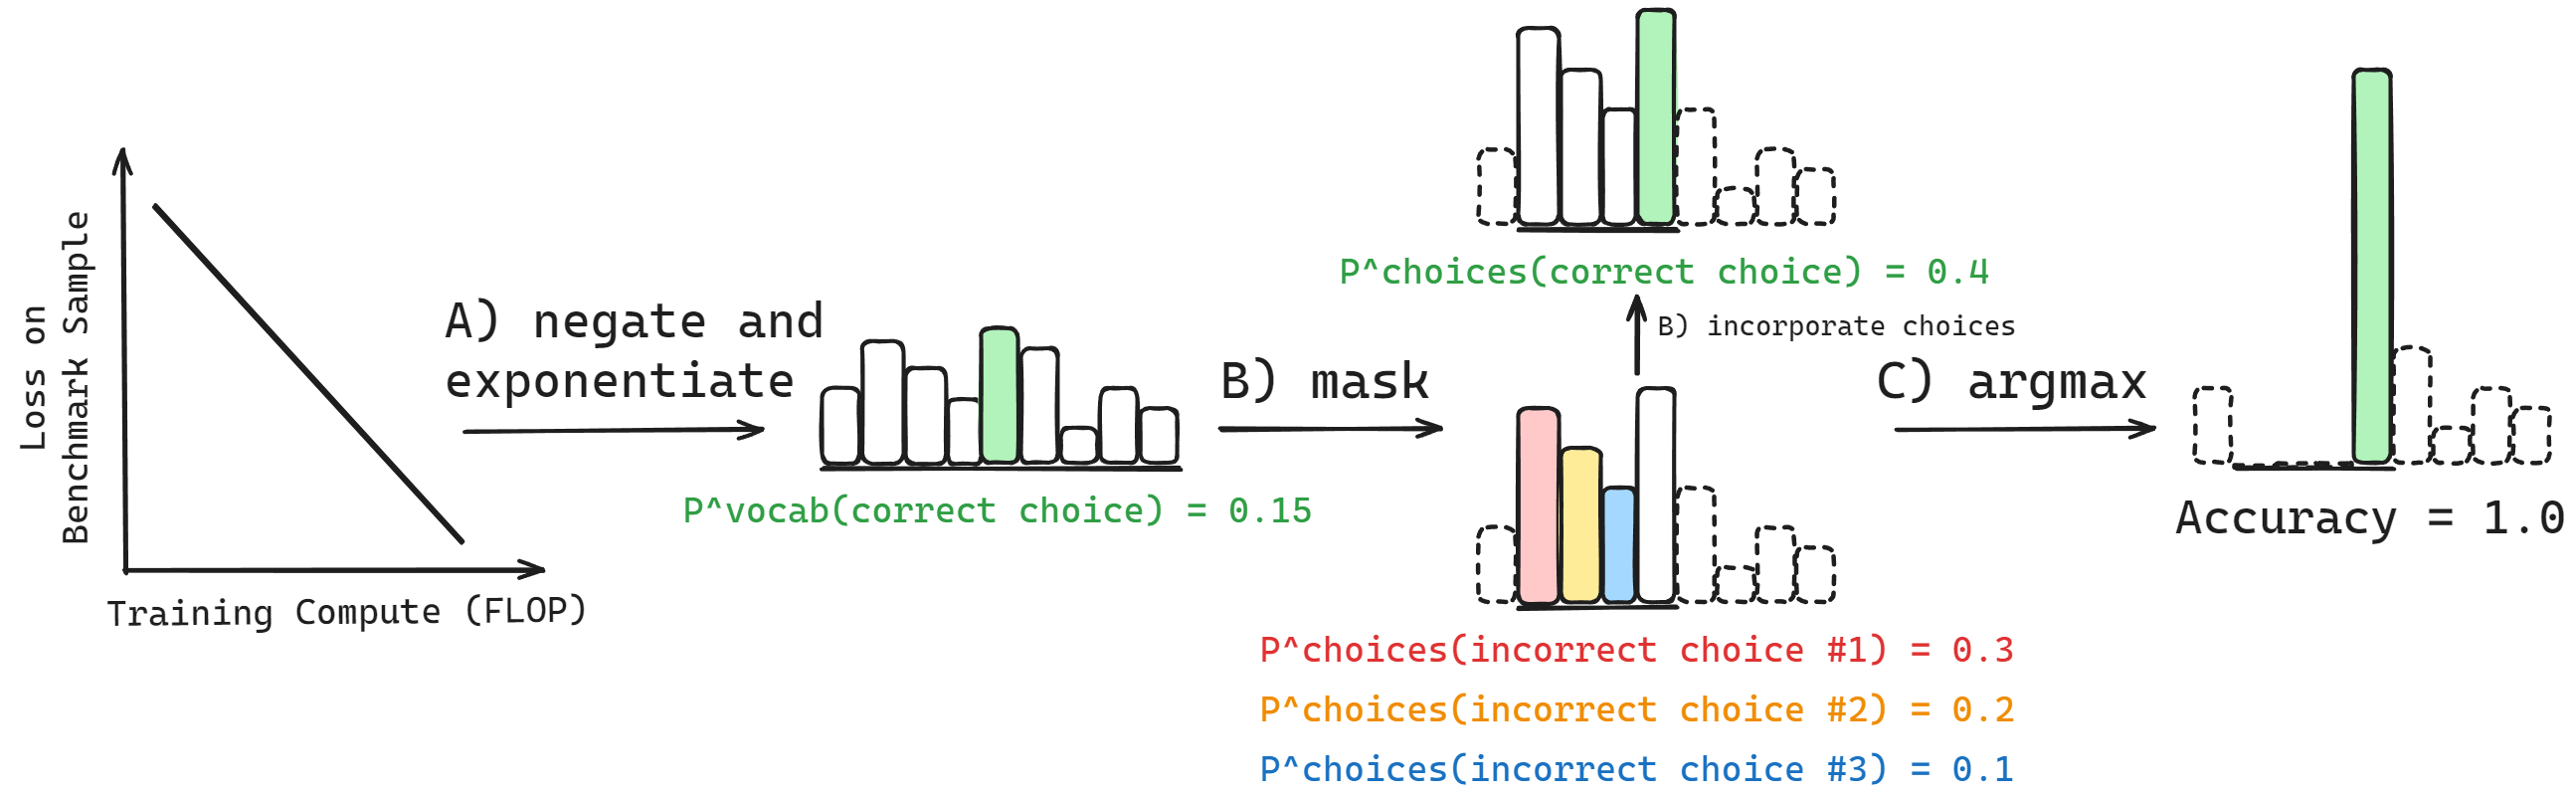
\includegraphics[width=\textwidth]
    {figures/schematics/Transformations_v10.png}
    \caption{\textbf{Multiple-choice benchmark accuracy is computed from negative log likelihoods via a sequence of transformations that degrades predictability.} 
    Computing \texttt{Accuracy} begins with computing the negative log likelihoods of each choice, then negating and exponentiating each to obtain the probability of each choice (\textbf{A}). Choices are then restricted to a set of available choices by \textit{masking} invalid continuations, and renormalizing to obtain relative probability mass on each choice (\textbf{B}).
    Lastly, the model's choice is defined as $\argmax_{i} \{p^{\text{Choices}}(\text{Available Choice}_i) \}$, and \texttt{Accuracy} is 1 if and only if the model's choice is the correct choice (\textbf{C}).
    }
    \label{fig:transformations-schematic}
\end{figure*}

However, while scaling laws for pretraining loss are well-established \citep{hestness2017deep,rosenfeld2019constructive,henighan2020scaling,kaplan2020scaling,gordon2021data,hernandez2021scaling,jones2021scaling,zhai2022scaling,hoffmann2022training,clark2022unified,neumann2022scaling,hernandez2022scaling,maloney2022solvable,sardana2023chinchillaoptimal,muennighoff2024scaling,besiroglu2024chinchilla}, the literature is less conclusive regarding predicting specific downstream capabilities with scale.
Prior work has observed that performance on standard natural language processing (NLP) benchmarks can exhibit \textit{emergent abilities} \citep{brown2020language,ganguli2022predictability,srivastava2022beyond,wei2022emergent} where performance changes unpredictably with scale, but further work demonstrated that such unpredictable changes can be artifacts of researchers' analyses, i.e., choices of metrics and lack of sufficient resolution from too few samples \citep{srivastava2022beyond,schaeffer2023mirage,hu2024predicting}.
% More recently, Du et al. (2024) %\SK{Minor (and can ignore for deadline), but weird to write out refs. Strongly suggest using \texttt{citet} and \texttt{citep} primitives}
% claimed that downstream capabilities \textit{can} be predicted, but \textit{only} after the pretraining cross-entropy loss falls below a certain threshold \cite{du2024understanding}, and Gadre et al. (2024) claimed that while performance on individual tasks can be difficult to predict, aggregating results across a dozen or more diverse benchmarks leads to clearer scaling trends \cite{gadre2024language}.
More recently, \citet{du2024understanding} claim that downstream capabilities \textit{can} be predicted, but \textit{only} after the pretraining cross-entropy loss falls below a certain threshold, and \citet{gadre2024language} claim that while performance on individual tasks can be difficult to predict, aggregating results across dozens of diverse benchmarks yields clearer scaling trends. In this work, we ask: in contrast with strongly-predictable pretraining losses, \textit{why has predicting specific downstream capabilities with scale remained elusive?}



\section{Contribution: Explaining Why Predicting Downstream Capabilities With Scale Has Remained Elusive}

Our goal is to understand what breaks down between the predictability of pretraining losses and the unpredictability of downstream evaluations. To do this, we investigated the comparative predictability of different evaluation methodologies and setups, focusing on popular and comparatively simple (yet still highly difficult to predict) multiple-choice question answering benchmarks. 
We began with scaling-predictable pretraining log likelihoods %$\log p^{\text{Vocab}}(\text{Correct Choice})$ 
and tracked how these log likelihoods are transformed in the process of calculating downstream evaluation metrics that are notoriously difficult to predict, such as \texttt{Accuracy} or \texttt{Brier Score} (See Fig. \ref{fig:transformations-schematic} and Sec. \ref{sec:what_makes} for further details):
%
\begin{equation*}
\begin{aligned}
    &\underbrace{\log p_{\theta}^{\text{Vocab}}(\text{Correct Choice})}_{\text{Scaling-Predictable}}\\
    &\quad\quad\quad\quad \rightarrow p_{\theta}^{\text{Vocab}}(\text{Correct Choice})\\
    &\quad\quad\quad\quad\quad\quad\quad\quad \rightarrow p_{\theta}^{\text{Choices}}(\text{Correct Choice})\\
    &\quad\quad\quad\quad\quad\quad\quad\quad\quad\quad\quad\quad \rightarrow \underbrace{\texttt{Accuracy}}_{\text{Scaling-Unpredictable}}
\end{aligned}
\end{equation*}
%
This paper demonstrates the following findings:
%
\begin{enumerate}
    \item \textbf{Calculating downstream metrics requires a sequence of transformations applied to the original scaling-predictable quantities. These transformations progressively deteriorate the statistical relationship between those metrics and the scaling parameters (parameters, data, and compute).} This formalizes an intuition that ``more complex'' metrics might be less easily predictable.
    \item 
    \textbf{Accurately predicting downstream multiple-choice performance requires modeling not only the probability mass assigned to the correct choice with scale, but also the probability mass assigned to the incorrect alternatives.} This explains the cause of comparative unpredictability of multiple-choice benchmarks; it also suggests a potential path forward for successful predictive models of downstream performance in the area of multiple-choice question answering, and in general the need to model \textit{external information} not related to scaling-predictable log likelihoods needed for downstream metric computation.
    \item \textbf{Continuous metrics such as \texttt{Brier Score} are insufficient for recovering predictability.} We observe that, contrary to prior work showing that metrics such as \texttt{Brier Score} can hide \textit{emergent behavior} at times, \texttt{Brier Score} is insufficient to improve the statistical relationship degraded by incorporating incorrect choices' probability mass.
\end{enumerate}

% Our findings explain that the apparent unpredictability of individual downstream evaluations is due to alternative incorrect choices, which the strongly predictable pretraining losses do not depend upon.
% More broadly, we argue that a precise understanding of the factors affecting downstream performance is essential for designing evaluations to reliably track the progression of frontier AI models' capabilities.
